% ****** Start of file apssamp.tex ******
%
%   This file is part of the APS files in the REVTeX 4.1 distribution.
%   Version 4.1r of REVTeX, August 2010
%
%   Copyright (c) 2009, 2010 The American Physical Society.
%
%   See the REVTeX 4 README file for restrictions and more information.
%
% TeX'ing this file requires that you have AMS-LaTeX 2.0 installed
% as well as the rest of the prerequisites for REVTeX 4.1
%
% See the REVTeX 4 README file
% It also requires running BibTeX. The commands are as follows:
%
%  1)  latex apssamp.tex
%  2)  bibtex apssamp
%  3)  latex apssamp.tex
%  4)  latex apssamp.tex
%
\documentclass[%
 reprint,
%superscriptaddress,
%groupedaddress,
%unsortedaddress,
%runinaddress,
%frontmatterverbose,
%preprint,
%showpacs,preprintnumbers,
%nofootinbib,
%nobibnotes,
%bibnotes,
 amsmath,amssymb,
 aps,
pra,
%prb,
%rmp,
%prstab,
%prstper,
%floatfix,
]{revtex4-1}

\usepackage{graphicx}% Include figure files
\usepackage{dcolumn}% Align table columns on decimal point
\usepackage{bm}% bold math
\usepackage{enumitem}
% Stuff for Mogens' nice figure
\usepackage{braket}
\usepackage{tikz}


% Stuff for showing the algorithms
\usepackage{algorithm}
\usepackage[noend]{algpseudocode}

\newcommand{\dif}[2]{\frac{\text{d} #1}{\text{d} #2}}
\newcommand{\diff}[2]{\frac{\partial #1}{\partial #2}}
\DeclareMathOperator*{\argmin}{arg\,min}

\newcommand{\procspie}{Proceedings of the SPIE}
%\usepackage{hyperref}% add hypertext capabilities
%\usepackage[mathlines]{lineno}% Enable numbering of text and display math
%\linenumbers\relax % Commence numbering lines

%\usepackage[showframe,%Uncomment any one of the following lines to test
%%scale=0.7, marginratio={1:1, 2:3}, ignoreall,% default settings
%%text={7in,10in},centering,
%%margin=1.5in,
%%total={6.5in,8.75in}, top=1.2in, left=0.9in, includefoot,
%%height=10in,a5paper,hmargin={3cm,0.8in},
%]{geometry}

\begin{document}

%\preprint{APS/123-QED}

\title{Gradient-Based Optimal Control of Quantum Many-body Systems in Optical Lattices}% Force line breaks with \\

\author{J. J. W. H. S\o rensen}
\author{F. S. M\o ller}
\author{J. F. Sherson}
\affiliation{Aarhus University}
\email{sherson@phys.au.dk}
\date{\today}% It is always \today, today,
             %  but any date may be explicitly specified

\begin{abstract}
Abstract ...


\end{abstract}

\maketitle

\section{Introduction}

\section{Quantum Optimal Control}
In quantum optimal control a given state transfer or unitary is achieved by dynamically manipulating a system through a time-dependent Hamiltonian
\begin{equation}
	\hat{H} =  \hat{H}_0 + \sum_{n = 1}^{m}  \hat{H}_n (u_n(t)) \; ,
	\label{eq:ControlHamiltonians}
\end{equation} 
where $\hat{H}_0$ is an uncontrollable drift, while $\hat{H}_n$ can be adjusted through the control parameters $u_n(t)$. If a state transfer is desired, $\ket{\psi_0} \to \ket{\psi_{\mathrm{target}}}$, the optimal control problem can be written as the minimization of the cost function
\begin{equation}
	J = \frac{1}{2} \left( 1-|\braket{\psi_{\mathrm{target}} | \psi (T)}|^2 \right) \; ,
	\label{eq:infidelityCost}
\end{equation}
where $T$ is the duration of the control sequence. Thus, one must find the set of control parameters, which maximizes the overlap between the final state, $\ket{\psi (T)}$, and the target state.

A standard approach to finding the optimal control parameters is the GRAPE algorithm, which utilizes the gradient of the cost function to update the control. In GRAPE the control is discretized according to a time-step $\Delta t$ resulting in the optimization of $N = \lfloor T / \Delta t \rfloor$ parameters \cite{khaneja2005optimal}. While the gradient of the cost functional in the original algorithm was derived to $O(\Delta t ^2)$ precision, a series of higher order corrections were added in \cite{de2011second}. The derivative of the cost function \eqref{eq:infidelityCost} with respect to the time-discretized control parameters is
\begin{equation}
	\frac{\partial J}{\partial u_n (t_j)}  = - \Re \Braket{\chi (t_j) | i  \frac{\partial \hat{\mathcal{U}}_{t_j}}{\partial u_n (t_j)} | \psi (t_{j-1})} \; , \label{eq:CostDeriv}
\end{equation}
where $\ket{\chi (T)} \equiv i \ket{\psi_{\mathrm{target}}} \braket{\psi_{\mathrm{target}} | \psi (T)}$ must be propagated back in time to obtain $\ket{\chi (t_j)}$.
The derivative of the propagator with respect to the control is given by
\begin{align}
	\frac{\partial \hat{\mathcal{U}}_{j}}{\partial u_n (t_j)} &= e^{-i \hat{H} (u_n (t_j)) \Delta t} \nonumber \\ 
	 \times \sum_{k = 0}^{\infty } &  \frac{i^{k-1} \Delta t^{k+1}}{(k+1)!} \left[ \hat{H} (u_n (t_j)) , \frac{\partial \hat{H} (u_n (t_j))}{\partial u_n (t_j)}  \right]_k \; , \label{eq:PropDeriv}
\end{align}
where the zeroth order term of the recursive commutator produces the gradient of the original GRAPE algorithm.

Since the control function, and thereby the Hamiltonian, is repeatedly modified during the optimization procedure, the propagator most be re-calculated multiple times. This is costly, as exponentiating the Hamiltonian is a non-trivial operation. Non-updated parts of the propagator can be re-used, by expanding the propagator through the Suzuki-Trotter expansion 
\begin{equation}
		e ^{( \hat{H}_n + \hat{H}_0  ) \delta } = e^{  \hat{H}_n \delta /2  } e^{ \hat{H}_0 \delta } e^{ \hat{H}_n \delta /2 } + O(\delta^3) \; . \label{eq:SuzukiTrotter}
\end{equation}
Calculating the propagator can be done very efficiently, if the controllable part of the Hamiltonian is diagonal. Thereby, the repeated exponentiation is trivial, while constant, non-diagonal parts of the Hamiltonian can be exponentiated separately at the start of the optimization.

Consider the Suzuki-Trotter expansion of eq. \eqref{eq:SuzukiTrotter}, where the Hamiltonian $\hat{H}_n$ is diagonal. Additional accuracy can be achieved by evaluating $\hat{H}_n$ using the midpoint rule, i.e. when evolving the state from $t_{j-1} \to t_j$ propagate first using $\hat{H}_n (u (t_{j-1}))$ followed by $\hat{H}_n (u (t_{j}))$ at the end of the expansion. Utilizing the midpoint rule along with the Suzuki-Trotter expansion also has profound impact on the  gradient, as all higher-order contributions vanish.
Expressing the Suzuki-Trotter expanded propagator as
\begin{align}
	\hat{\mathcal{U}}_{j}^{\mathrm{ST}} &= e^{ -i  \hat{H}_n (u (t_j)) \Delta t /2 } \; e^{ -i \hat{H}_0 \Delta t } \; e^{ -i  \hat{H}_n (u (t_{j-1}))  \Delta t /2 } \\
	& \equiv \hat{\mathcal{U}}_{j}^{(n)} \hat{\mathcal{U}}_{j}^{(0)} \hat{\mathcal{U}}_{j-1}^{(n)} \; , 
\end{align}
makes it clear that both $\mathcal{U}_{j}^{\mathrm{ST}}$ and $\mathcal{U}_{j+1}^{\mathrm{ST}}$ contribute to the cost derivative.
The derivative of $\mathcal{U}_{j}^{\mathrm{ST}}$ according to eq. \eqref{eq:PropDeriv} is
\begin{align}
	\frac{\partial \hat{\mathcal{U}}_{j}^{\mathrm{ST}}}{\partial u_n (t_j)} &=  \frac{\partial \hat{\mathcal{U}}_{j}^{(n)}}{\partial u_n (t_j)} \hat{\mathcal{U}}_{j}^{(0)} \hat{\mathcal{U}}_{j-1}^{(n)} \nonumber \\
	&= e^{ -i  \hat{H}_n (u (t_j)) \Delta t /2 } \left( -i \hat{H}_n (u_n (t_j)) \Delta t /2 \right) \hat{\mathcal{U}}_{j}^{(0)} \hat{\mathcal{U}}_{j-1}^{(n)} \nonumber \\
	&= \left( -i \hat{H}_n (u_n (t_j)) \Delta t /2 \right) \hat{\mathcal{U}}_{j}^{\mathrm{ST}} \; . \label{eq:STpropderiv1}
\end{align}
Since $\hat{H}_n$ is diagonal, the recursive commutator is vanishing for $k > 0$, which causes all higher-order contributions to the derivative of the propagator to drop out.\\
Likewise, the derivative of the second propagator is
\begin{equation}
	\frac{\partial \hat{\mathcal{U}}_{j+1}^{\mathrm{ST}}}{\partial u_n (j)} =  \hat{\mathcal{U}}_{j+1}^{\mathrm{ST}} \left( -i \hat{H}_n (u_n (t_j)) \Delta t /2 \right) \; . \label{eq:STpropderiv2}
\end{equation}
Inserting the derivatives of eq. \eqref{eq:STpropderiv1} and \eqref{eq:STpropderiv2} into the derivative of the cost (eq. \eqref{eq:STcostderiv}) yields
\begin{align}
	\frac{\partial J}{\partial u_n (t_j)} &= - \Re \Braket{\chi (t_j) |  \left(  \hat{H}_n (u_n (t_j)) \Delta t /2 \right) \hat{\mathcal{U}}_{j}^{\mathrm{ST}} | \psi (t_{j-1})} \nonumber \\
	& \quad - \Re \Braket{\chi (t_{j+1}) | \hat{\mathcal{U}}_{j+1}^{\mathrm{ST}} \left(  \hat{H}_n (u_n (t_j)) \Delta t /2 \right) | \psi (t_{j})} \nonumber \\
	&= - \Re \Braket{\chi (t_j) | \hat{H}_n (u_n (t_j)) \Delta t | \psi (t_{j})} \; . \label{eq:STcostgrad}
\end{align}  
Thus, the combination of the Suzuki-Trotter expansion and a diagonal control Hamiltonian eliminates all higher order contributions to the gradient. Thereby, the gradient of the cost is exact up to the order of the expansion.

In GRAPE the dimension of the optimization space is $N = \lfloor T / \Delta t \rfloor$ due to the discretization. However, most optimal solutions require much fewer degrees of freedom than introduced in the discretization. Therefore, expanding the control in a proper basis can significantly reduce the dimension of the optimization space.
The GROUP algorithm utilizes the gradient-based optimization from GRAPE while employing a chopped basis parametrization 
\begin{equation}
	u(t) = u_0 (t) + S(t) \sum_{n=1}^{M} c_n f_n (t) \; . \label{eq:controlParametrization}
\end{equation}
Here, $f_n$'s are basis functions, the coefficients $c_n$'s are the optimization parameters, $u_0 (t)$ is the initial seed, and $S(t)$ is a shape function enforcing the boundary conditions of the original control. The derivative of the cost function in the parameterization can be derived using the chain rule
\begin{equation}
	\frac{\partial J }{\partial c_n} = \sum_{j = 1}^{N} \frac{\partial J }{\partial u(t_j)} S(t_j) f_n(t_j) \; . \label{eq:GROUPgradient} 
\end{equation}
The cost of calculating the partial derivative of eq. \eqref{eq:GROUPgradient} is dominated by the time evolution of the states $\psi$ and $\chi$ from eq. \eqref{eq:CostDeriv}. Hence, the computation time of the parametrized gradient is comparable to that of GRAPE.

Optimal control problem often involve constraints ensuring the control parameters stay within a feasible limit
\begin{equation}
	 u_{min} (t_j) \leq u(t_j) \leq u_{max} (t_j) \; .
	 \label{eq:ControlConstraints}
\end{equation}
The parameterizing of eq. \eqref{eq:controlParametrization} does not alter the constraints, although additional constraints of the $c_n$ coefficients can be introduced. However, optimizing a constrained problem through its gradient requires the derivatives of the constraints expressed through a Jacobian, which will be affected by the parameterization. The matrix elements of the Jacobian of eq. \eqref{eq:ControlConstraints} parametrized by \eqref{eq:controlParametrization} are
\begin{equation}
	\boldsymbol{J}_{ij} = \frac{\partial u(t_i)}{\partial c_j} = S(t_i) f_j (t_i) \; . \label{eq:ConstraintJacobian}
\end{equation}
The Jacobian of the constraints has $N \times M$ entries, which remains constant throughout the optimization, whereby they can easily be retrieved.
  

\section{Results}


\begin{figure}[h!]
    \centering
    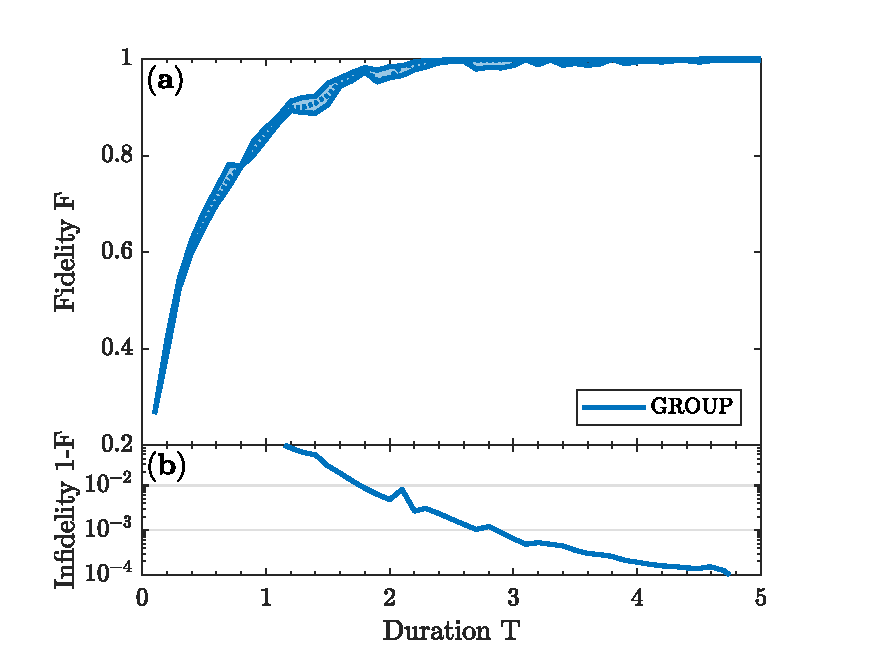
\includegraphics[width=0.45\textwidth]{Figures/FidelityDuration.pdf}
    \caption{\textit{Final fidelity obtained for optimal control at various durations. \textbf{(a)} the dotted line marks the median fidelity achieved, while the shaded area displays the $25\%$- and $75\%$-quartiles of the solutions. \textbf{(b)} the lowest infidelity achieved for each duration. }}
    \label{fig:FidelityDuration}
\end{figure}

\begin{figure}[h!]
    \centering
    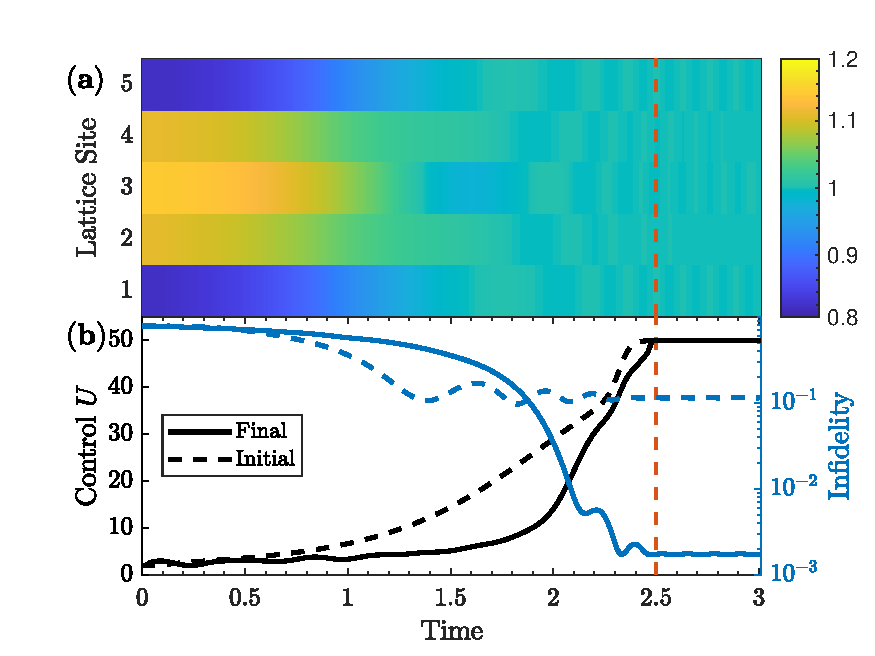
\includegraphics[width=0.45\textwidth]{Figures/OptRamp.pdf}
    \caption{\textit{Solution with highest fidelity achieved for duration $T = 2.5$. The dashed, red line marks the end of the duration, from which the system is further evolved using the final control value. \textbf{(a)} logarithmically scaled expectation value of the number operator, $\braket{\hat{n}_i}$, for each site, as the system is evolved according to the optimized ramp. \textbf{(b)} the initial and optimized ramp sequences along with the corresponding evolution of fidelities.}}
    \label{fig:OptRamp}
\end{figure}

\begin{figure}[h!]
    \centering
    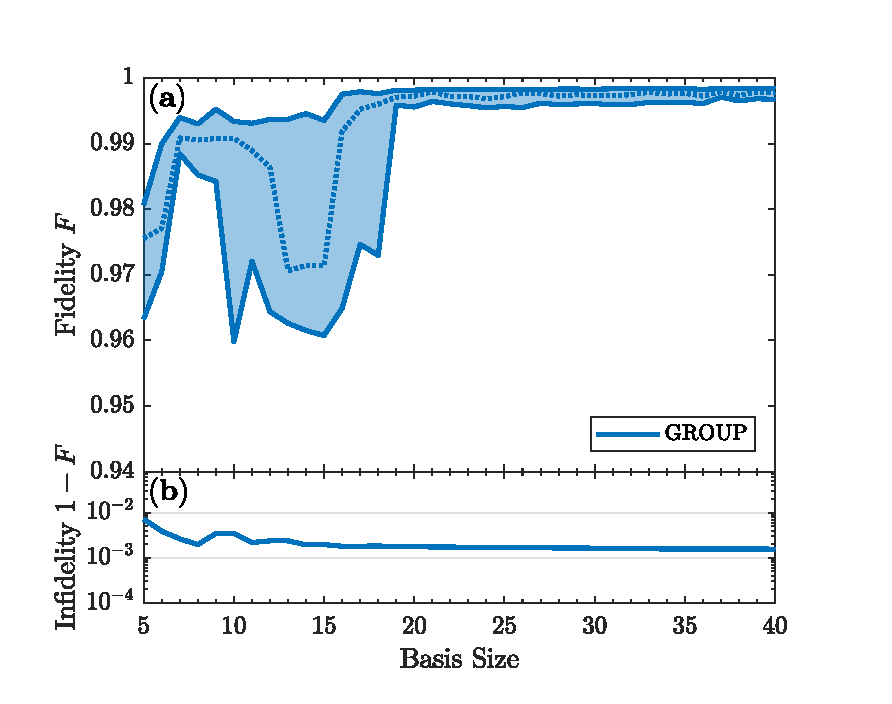
\includegraphics[width=0.45\textwidth]{Figures/FidelityBasisSize.pdf}
    \caption{\textit{Final fidelity obtained for optimal control at various optimization space dimensions for duration $T = 2.5$. \textbf{(a)} the dotted line marks the median fidelity achieved, while the shaded area displays the $25\%$- and $75\%$-quartiles of the solutions. \textbf{(b)} the lowest infidelities achieved for each basis size.}}
    \label{fig:FidelityBasisSize}
\end{figure}

\begin{figure}[h!]
    \centering
    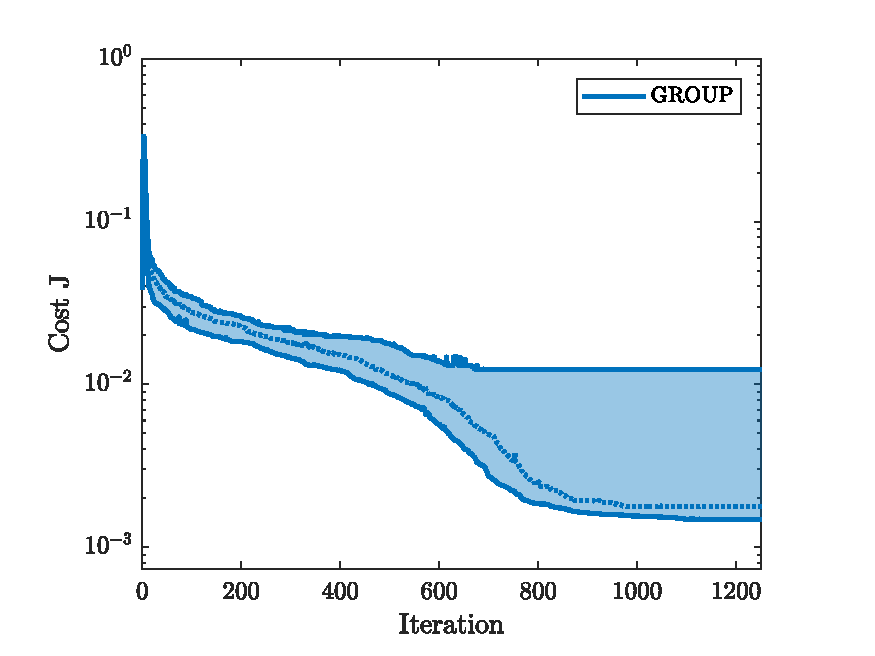
\includegraphics[width=0.45\textwidth]{Figures/CostProgress.pdf}
    \caption{\textit{The value of the cost function at a given number of time evolutions. The dotted line marks the median and the shaded area indicates the $25\%$- and $75\%$-quartiles found from X different random initial controls.}}
    \label{fig:FidelityBasisSize5}
\end{figure}


%\bibliographystyle{apsrev4-1}
\bibliography{references.bib}

\end{document}
%
% ****** End of file apssamp.tex ******
